% !TeX spellcheck = ru_RU
% !TEX root = vkr.tex

\section{Эксперимент}
\label{sec:experiment}
% Как мы проверяем, что всё удачно получилось.
% Если работа рассчитана на несколько семестров и в текущем до эксперимента дело не дошло, опишите максимально подробно, как он будет прово\-диться и на чём
% (то, что называется \emph{дизайн эксперимента}~--- от того, что и как Вы будете проверять, очень сильно зависит, что Вы будете делать, так что это важно и делается \emph{не} после реализации).

В данном разделе описаны эксперименты по обучению модели, замеру метрик детекции и
end-to-end метрик.

\subsection{Условия эксперимента}
% Железо (если актуально);
% версии ОС, компиляторов и параметры командной строки;
% почему мы выбрали именно эти тесты; входные дан\-ные, на которых проверяем наш подход, и почему мы выбрали именно их.

Эксперимент по обучению модели \texttt{YOLO} проводился на платформе \texttt{kaggle}.
Технические характеристики указаны ниже:
\begin{itemize}
    \item CPU: Intel Xeon 2.00 GHz
    \item CPU count: 4
    \item GPU: NVIDIA Tesla T4 16 GB
    \item GPU count: 2
    \item RAM: 31.35 GB
\end{itemize}

\subsection{Исследовательские вопросы}
% По-английски называется \emph{research questions}, в тексте можно ссылаться на них как RQ1, RQ2, и т.~д.
% Необходимо сформулировать, чего мы хотели бы добиться работой (2 пункта будет хорошо):

В ходе экспериментов нужно было ответить на следующие исследовательские вопросы.

\begin{description}
    \item[RQ1]: позволяет ли предложенный подход получить качественные end-to-end-метрики?
\end{description}

% Иногда в работах это называют гипотезами, которые потом проверяют.
% Далее в тексте можно ссылаться на исследовательские вопросы как \textsc{RQ}, это обще\-при\-нятое сокращение.

\subsection{Метрики}

В работе использовались известные метрики для задачи детекции: \texttt{mAP50}, \texttt{mAP50-90},
\texttt{precision}, \texttt{recall}, \texttt{F1}. Все перечисленные метрики применяются для оценки качества детекции.

В качестве end-to-end-метрики использовалась пользовательская метрика доли пропущенных строк.
Для работников и техники \texttt{MAPE} вычислялась как абсолютная относительная ошибка среднего количества объектов:
\[
    \texttt{MAPE} =
    \frac{\left|\overline{x}_{\text{исх.}} - \overline{x}_{\text{пред.}}\right|}
    {\overline{x}_{\text{исх.}}} \cdot 100\%.
\]

% Как мы сравниваем, что результаты двух подходов лучше или хуже:
% \begin{itemize}
%     \item Производительность.
%     \item Строчки кода.
%     \item Как часто алгоритм \enquote{угадывает} правильную класси\-фикацию входа.
% \end{itemize}

% \noindent Иногда метрики вырожденные (да/нет), это не очень хорошо, но если в области исследований так принято, то ладно.
% Если метрики хитрые (даже IoU или $F_1$-меру можно считать хитрыми), разберите их в обзоре, пояснив, почему выбраны именно такие метрики.

\subsection{Результаты}
\label{subsec:experiment-results}

\subsubsection{Результаты обучения модели YOLO}
\label{subsubsec:yolo-training-results}

Значения гиперпараметров и других настроек для обучения модели находятся в файле
\texttt{/models/yolo\_training.ipynb}.

\begin{table}[H]
    \centering
    \caption{Метрики модели YOLO после дообучения}
    \label{tab:yolo-finetuning-metrics}
    \begin{tabular}{*{4}{S[table-format=1.3]}}
        \toprule
        {Precision} & {Recall} & {mAP50} & {mAP50-90} \\
        \midrule
        0.879 & 0.720 & 0.812 & 0.601 \\
        \bottomrule
    \end{tabular}
\end{table}

\begin{figure}[H]
    \centering
    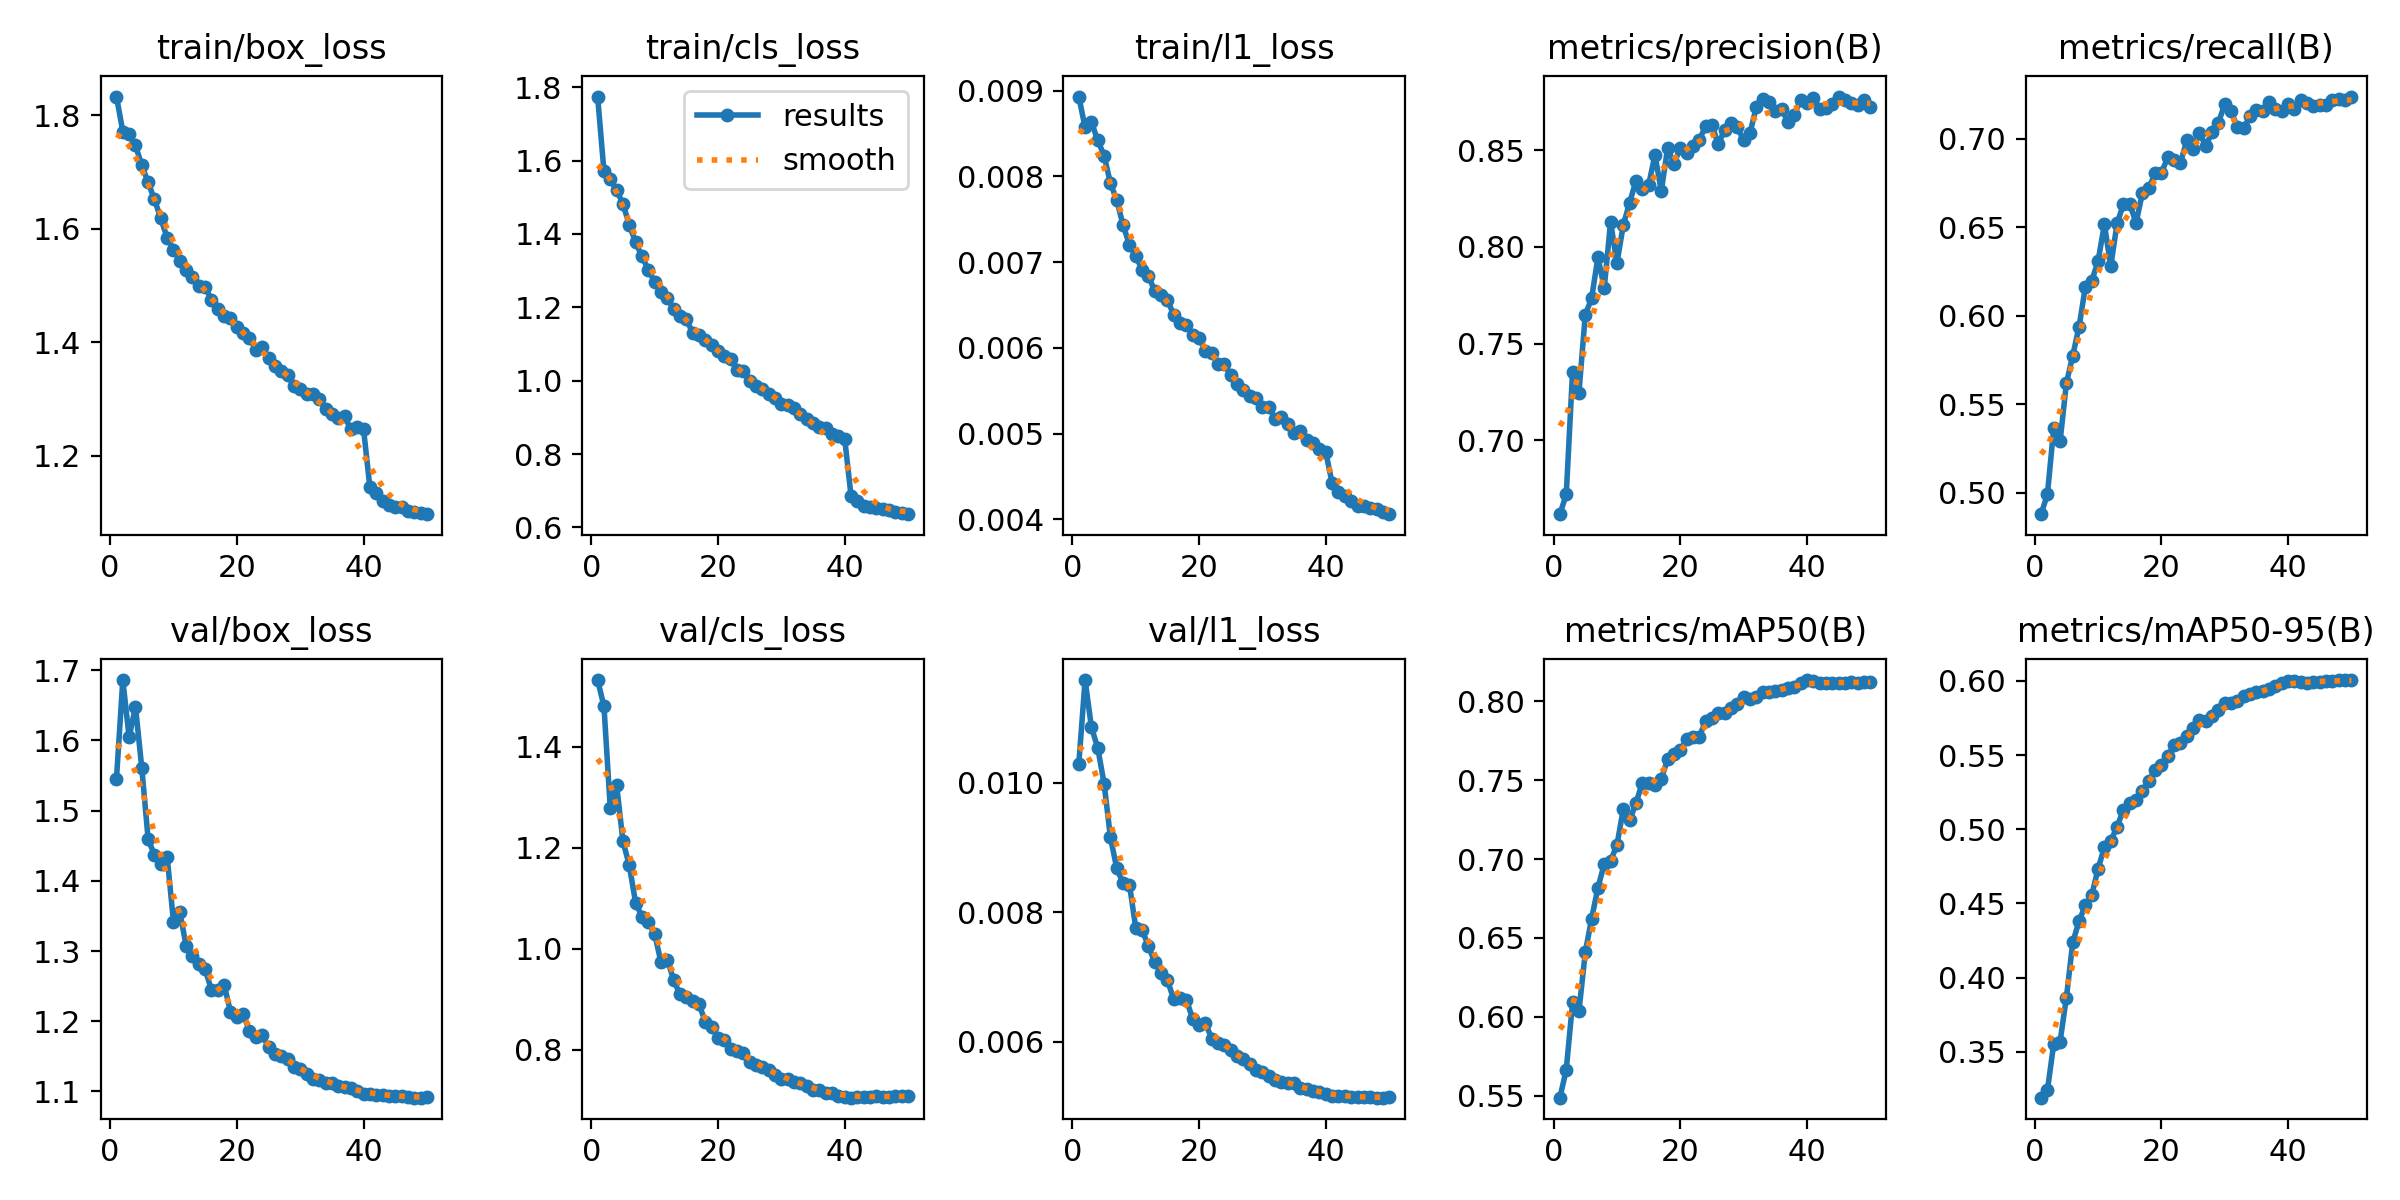
\includegraphics[width=0.9\textwidth]{figures/losses.png}
    \caption{Динамика функции потерь при обучении YOLO и значения метрик}
    \label{fig:yolo-finetuning-losses}
\end{figure}

\begin{figure}[H]
    \centering
    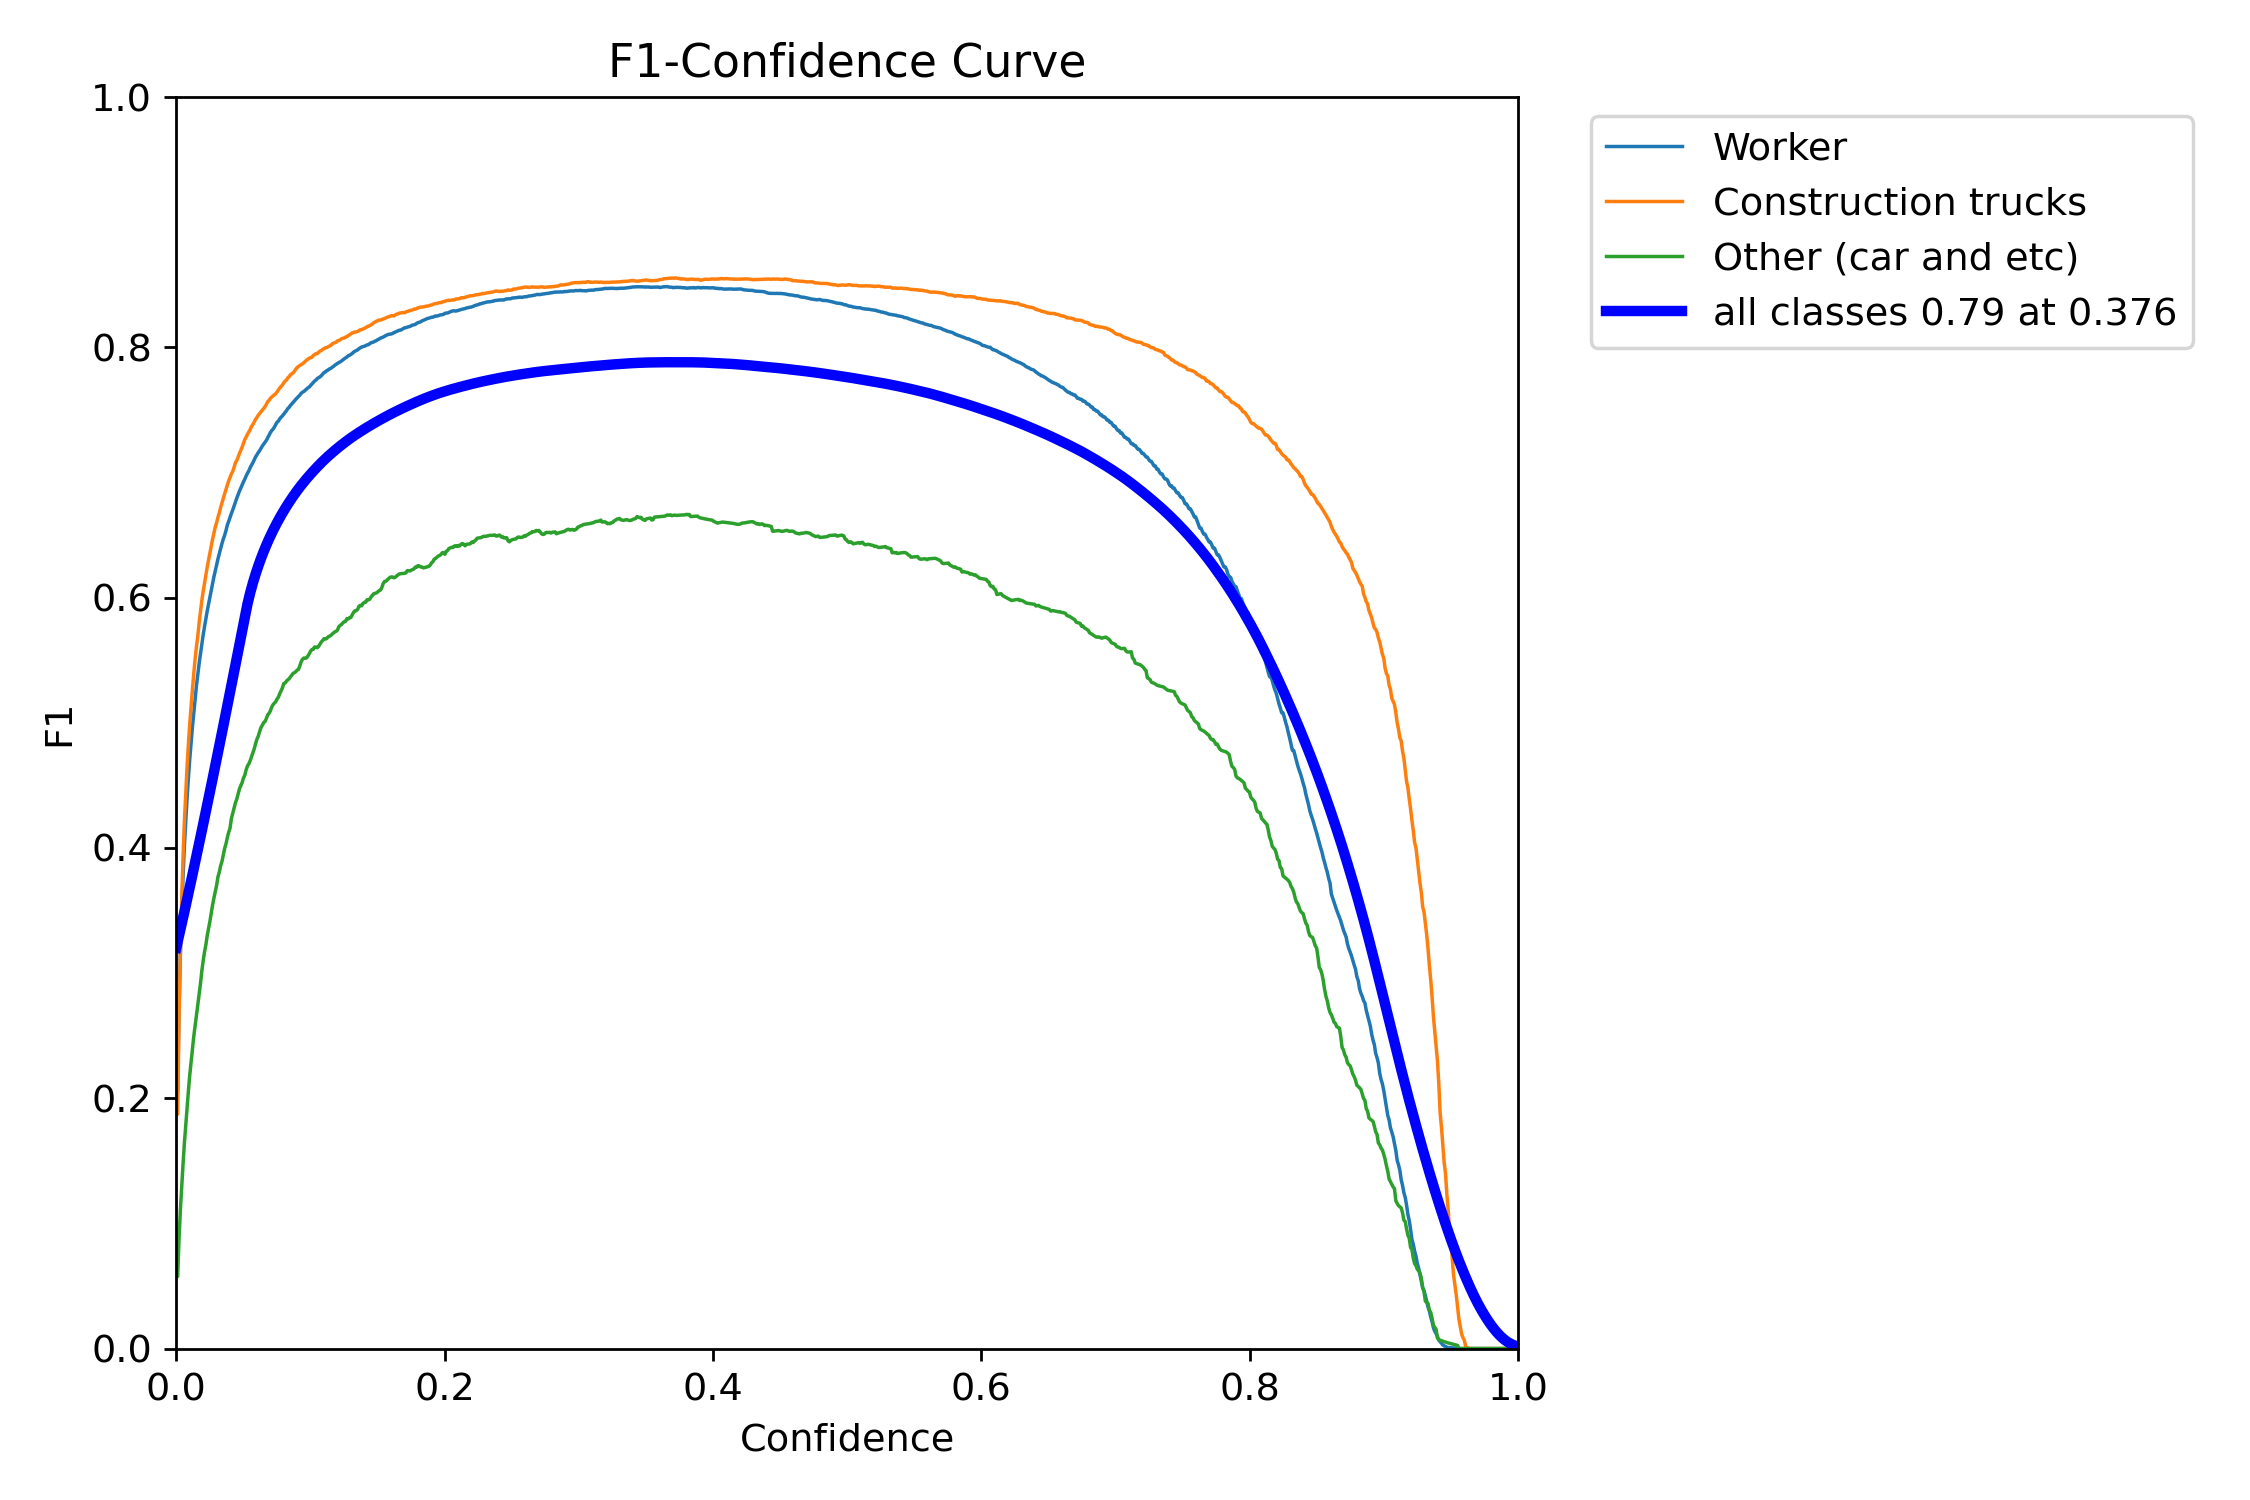
\includegraphics[width=0.9\textwidth]{figures/F1.png}
    \caption{Зависимость F1-меры от порога уверенности модели YOLO}
    \label{fig:yolo-finetuning-f1}
\end{figure}

\begin{figure}[H]
    \centering
    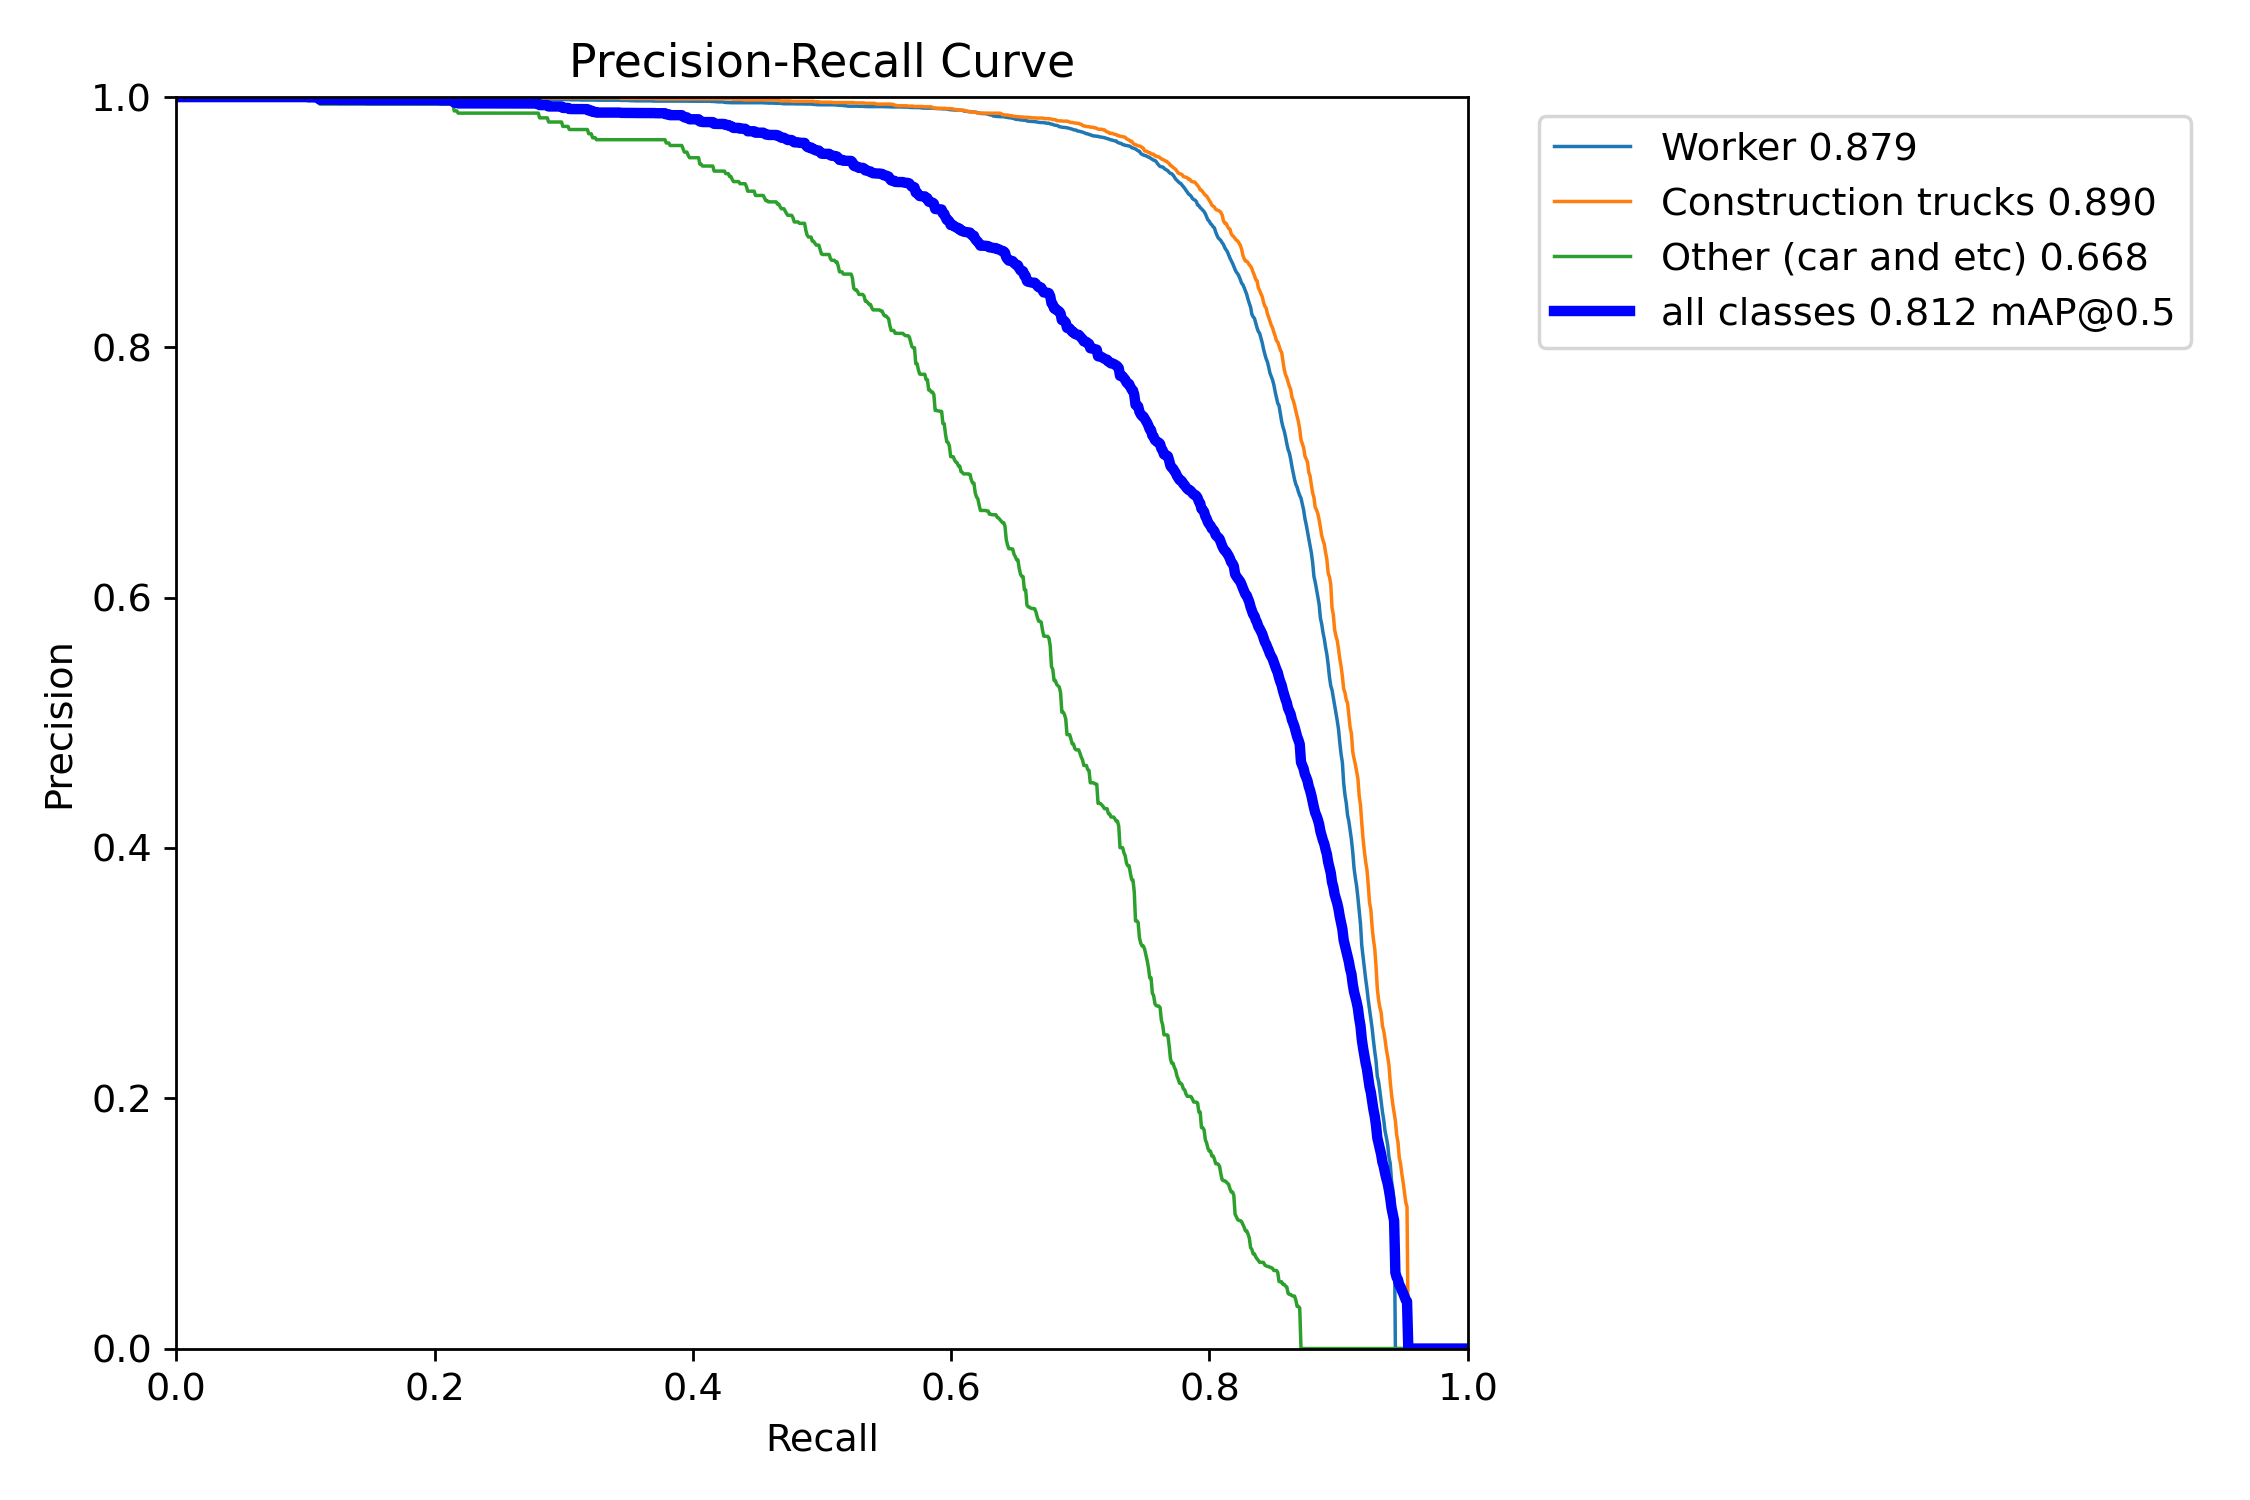
\includegraphics[width=0.9\textwidth]{figures/PR.png}
    \caption{Кривая precision-recall модели YOLO после дообучения}
    \label{fig:yolo-finetuning-pr}
\end{figure}

\subsubsection{Результаты замера end-to-end метрик}

Эксперимент проводился на трёх тестовых видео; исходные и предсказанные данные находятся в репозитории в директории \texttt{metrics}.



\begin{table}[H]
    \centering
    \caption{Результаты замера end-to-end метрик}
    \label{tab:end-to-end-metrics}
    \begin{tabular}{c c c S[table-format=2.2] S[table-format=2.2] S[table-format=2.2]}
        \toprule
        Смена &
        \makecell{Работники\\исх./пред.} &
        \makecell{Техника\\исх./пред.} &
        {\makecell{Доля\\пропусков,\\\%}} &
        {\makecell{MAPE\\работников,\\\%}} &
        {\makecell{MAPE\\техники,\\\%}} \\
        \midrule
        0001 & 9.26 / 9.23 & 0.85 / 0.85 & 4.38 & 0.32 & 0.01 \\
        0002 & 12.32 / 12.30 & 1.63 / 1.57 & 5.16 & 0.21 & 3.62 \\
        0003 & 6.11 / 5.68 & 2.12 / 2.12 & 4.72 & 7.04 & 0.00 \\
        \bottomrule
    \end{tabular}
\end{table}

% Результаты понятно что такое.
% Тут всякие таблицы и графики, как в таблице \ref{time_cmp_obj_func}.
% Обратите внимание, как цифры выровнены по правому краю, названия по центру, а разделители $\times$ и $\pm$ друг под другом.

% Перед написанием данного раздела имеет смысл проконсультироваться с литературой по проведению экспериментов~\cite{SmirnovCheatsheet}.

% Скорее всего Ваши измерения будут удовлетворять нормальному распределению, в идеале это надо проверять с помощью критерия Кол\-могорова и т.п.
% Если критерий этого не подтверждает, то у Вас что-то сильно не так с измерениями, надо проверять кэши процессора, отключать Интернет во время измерений, подкручивать среду исполне\-ния (англ. runtime), что\-бы сборка мусора не вмешивалась и т.п.
% Если критерий удовлетворён, то необходимо либо указать мат. ожидание и доверительный/предсказы\-вающий интервал, либо мат. ожидание и среднеквадратичное отклонение, либо, если совсем лень заморачиваться, написать, что все измерения проводились с погрешностью, например, в 5\%.
% Не приводите слишком много значащих цифр (например, время работы в 239.1 секунды при среднеквадратичном отклонении в 50 секунд выглядит глупо, даже если ваш любимый бенчмарк так посчитал).

% Замечание: если у вас получится улуч\-шение производительности в пределах погреш\-ности, то это обязательно вызовет вопросы.
% Если погрешность получилась значительной (больше 10-15\% от среднего), это тоже вызовет вопросы, на которые надо ответить, либо разобравшись, что не так (первый подозреваемый~--- мультимодальное распределение), либо более глубоко статистически проанализировав результаты (например, привести гистограммы).

% В этом разделе надо также явно ответить на Research Questions или как-то их прокомментировать.

% \begin{table}
%     \def\arraystretch{1.1}  % Растяжение строк в таблицах
%     \setlength\tabcolsep{0.2em}
%     \centering
%     % \resizebox{\linewidth}{!}{%
%     \caption{Производительность какого-то алгоритма при различных разрешениях картинок  (меньше~--- лучше), в мс.,  CI=0.95. За пример таблички кидаем чепчики в честь Я.~Кириленко}
%     \begin{tabular}[C]{
%             S[table-format=4.4,output-decimal-marker=\times]
%             *4{S
%                         [table-figures-uncertainty=2, separate-uncertainty=true, table-align-uncertainty=true,
%                             table-figures-integer=3, table-figures-decimal=2, round-precision=2,
%                             table-number-alignment=center]
%                 }
%         }
%         \toprule
%         \multicolumn{1}{r}{Resolution} & \multicolumn{1}{r}{\textsc{TENG}} & \multicolumn{1}{r}{\textsc{LAPM}} &
%         \multicolumn{1}{r}{\textsc{VOLL4}} \\ \midrule
%         1920.1080 & 406.23 \pm 0.94 & 134.06 \pm 0.35 & 207.45 \pm 0.42  \\ \midrule
%         1024.768  & 145.0 \pm 0.47  & 39.68 \pm 0.1   &  52.79  \pm 0.1 \\ \midrule
%         464.848   & 70.57 \pm 0.2   & 19.86 \pm 0.01     & 32.75  \pm 0.04 \\ \midrule
%         640.480   & 51.10 \pm 0.2   & 14.70 \pm 0.1 & 24  \pm 0.04 \\ \midrule
%         160.120   & 2.4 \pm 0.02    & 0.67 \pm 0.01      & 0.92  \pm 0.01 \\
%         \bottomrule
%     \end{tabular}%
%     %}
%     \label{time_cmp_obj_func}
% \end{table}

% \clearpage
% % !TeX spellcheck = ru_RU
% !TEX root = vkr.tex

\newcolumntype{C}{ >{\centering\arraybackslash} m{4cm} }
\newcommand\myvert[1]{\rotatebox[origin=c]{90}{#1}}
\newcommand\myvertcell[1]{\multirowcell{5}{\myvert{#1}}}
\newcommand\myvertcelll[1]{\multirowcell{4}{\myvert{#1}}}
\newcommand\myvertcellN[2]{\multirowcell{#1}{\myvert{#2}}}

\afterpage{%
    \clearpage% Flush earlier floats (otherwise order might not be correct)
    \thispagestyle{empty}% empty page style (?)
    \begin{landscape}% Landscape page
        \centering % Center table

        \begin{tabular}{|c|c|c|c|c|c|c|c|c|c|c|c|c|c|c|c|c|c|}\hline
            %& \multicolumn{17}{c|}{} \\ \hline
            \multirowcell{2}{Код модуля \\в составе \\ дисциплины,\\практики и т.п. }
            &\myvertcellN{2}{Трудоёмкость\quad}
            & \multicolumn{10}{c|}{\tiny{Контактная работа обучающихся с преподавателем}}
            & \multicolumn{5}{c|}{\tiny{Самостоятельная работа}}
            & \myvertcellN{2}{\tiny Объем активных и интерактивных\quad}
            \\ \cline{3-17}

            && \myvertcellN{2}{лекции\quad}
            &\myvertcellN{2}{семинары\quad}
            &\myvertcellN{2}{консультации\quad}
            &\myvertcellN{2}{\small практические  занятия\quad}
            &\myvertcellN{2}{\small лабораторные работы\quad}
            &\myvertcellN{2}{\small контрольные работы\quad}
            &\myvertcellN{2}{\small коллоквиумы\quad}
            &\myvertcellN{2}{\small текущий контроль\quad}
            &\myvertcellN{2}{\small промежуточная аттестация\quad}
            &\myvertcellN{2}{\small итоговая аттестация\quad}

            &\myvertcellN{2}{\tiny под руководством    преподавателя\quad}
            &\myvertcellN{2}{\tiny в присутствии     преподавателя\quad}
            &\myvertcellN{2}{\tiny с использованием    методических\quad}
            &\myvertcellN{2}{\small текущий контроль\quad}
            &\myvertcellN{2}{\makecell{\small промежуточная \\ аттестация}}
            &     \\
            && &&&&&&&&& &&&&&&\\
            && &&&&&&&&& &&&&&&\\
            && &&&&&&&&& &&&&&&\\
            &&&&&&&&&&& &&&&&&\\
            &&&&&&&&&&& &&&&&&\\
            &&&&&&&&&&& &&&&&&\\ \hline
            Семестр 3 & 2 &30  &&&&&&&&2   & &&&18 &&20 &10\\ \hline
            &   &2--42&&&&&&&&2--25& &&&1--1&&1--1&\\ \hline
            Итого     & 2 &30  &&&&&&&&2   & &&&18 &&20 &10\\ \hline
        \end{tabular}

        \captionof{table}{Если таблица очень большая, то можно её изобразить на отдельной портретной странице. Не забудьте подробное описание, чтобы содержимое таблицы можно было понять не читая весь текст.}
    \end{landscape}
    \clearpage% Flush page
}



\subsubsection{RQ1}

Из таблицы \ref{tab:end-to-end-metrics} видно, что полученные end-to-end-метрики имеют приемлемые значения.
Это подтверждает возможность качественной работы сервиса.

\subsection{Выводы}

На данных строительной области модель может быть успешно обучена при использовании качественного набора данных.
Значения end-to-end-метрик приемлемы, но требуют дальнейшего улучшения. Для каждого домена данных модель можно дообучить,
и значения метрик станут лучше.

% Чуть более неформальное обсуждение, то, что сделано.
% Например, почему метод работает лучше остальных?
% Или, что делать со случаями, когда метод классифицирует вход некорректно.
